%% abtex2-modelo-projeto-pesquisa.tex, v-1 PFC 1 2016
%% Copyright 2012-2015 by abnTeX2 group at http://www.abntex.net.br/ 
%%
%% This work consists of the files abntex2-modelo-projeto-pesquisa.tex
%% and abntex2-modelo-references.bib
%%

% ------------------------------------------------------------------------
% ------------------------------------------------------------------------
% abnTeX2: Modelo de Projeto de pesquisa em conformidade com 
% ABNT NBR 15287:2011 Informação e documentação - Projeto de pesquisa -
% Apresentação 
% ------------------------------------------------------------------------ 
% ------------------------------------------------------------------------

\documentclass[
	% -- opções da classe memoir --
	12pt,				% tamanho da fonte
	openright,			% capítulos começam em pág ímpar (insere página vazia caso preciso)
	oneside,
    %twoside,			% para impressão em verso e anverso. Oposto a oneside
	a4paper,			% tamanho do papel. 
	% -- opções da classe abntex2 --
	%chapter=TITLE,		% títulos de capítulos convertidos em letras maiúsculas
	%section=TITLE,		% títulos de seções convertidos em letras maiúsculas
	%subsection=TITLE,	% títulos de subseções convertidos em letras maiúsculas
	%subsubsection=TITLE,% títulos de subsubseções convertidos em letras maiúsculas
	% -- opções do pacote babel --
	english,			% idioma adicional para hifenização
	french,				% idioma adicional para hifenização
	spanish,			% idioma adicional para hifenização
	brazil,				% o último idioma é o principal do documento
	]{abntex2}

% ---
% PACOTES
% ---

% ---
% Pacotes fundamentais 
% ---
\usepackage{lmodern}			% Usa a fonte Latin Modern
\usepackage[T1]{fontenc}		% Selecao de codigos de fonte.
\usepackage[utf8]{inputenc}		% Codificacao do documento (conversão automática dos acentos)
\usepackage{indentfirst}		% Indenta o primeiro parágrafo de cada seção.
\usepackage{color}				% Controle das cores
\usepackage{graphicx}			% Inclusão de gráficos
\usepackage{microtype} 			% para melhorias de justificação
% ---

% ---
% Pacotes adicionais, usados apenas no âmbito do Modelo Canônico do abnteX2
% ---
\usepackage{lipsum}				% para geração de dummy text
%\usepackage[num]{abntex2cite}
% ---

% ---
% Pacotes de citações
% ---
\usepackage[brazilian,hyperpageref]{backref}	 % Paginas com as citações na bibl
\usepackage[alf]{abntex2cite}	% Citações padrão ABNT

% --- 
% CONFIGURAÇÕES DE PACOTES
% --- 

% ---
% Configurações do pacote backref
% Usado sem a opção hyperpageref de backref
\renewcommand{\backrefpagesname}{Citado na(s) página(s):~}
% Texto padrão antes do número das páginas
\renewcommand{\backref}{}
% Define os textos da citação
\renewcommand*{\backrefalt}[4]{
	\ifcase #1 %
		Nenhuma citação no texto.%
	\or
		Citado na página #2.%
	\else
		Citado #1 vezes nas páginas #2.%
	\fi}%
% ---

% ---
% Informações de dados para CAPA e FOLHA DE ROSTO
% ---
\titulo{Patterns recognition and strategies for intervention in meaningful student learning, through EDM techniques and LA approaches}
\autor{Othon Luiz Teixeira de Oliveira}
\local{Recife -- PE}
\data{2017}
\tipotrabalho{Projeto de Pesquisa (Doutorado)}
% O preambulo deve conter o tipo do trabalho, o objetivo, 
% o nome da instituição e a área de concentração 
\preambulo{Pré-Projeto de Pesquisa apresentado ao programa de Pós-Graduação em Ciências da Computação da Universidade Federal de Pernambuco, como pré-requisito para seleção do programa de doutorado.}

\orientador {Prof. Dr. Alex Sandro Gomes}

\instituicao{Universidade Federal de Pernambuco - UFPE}


% ---

% ---
% Configurações de aparência do PDF final

% alterando o aspecto da cor azul
\definecolor{blue}{RGB}{41,5,195}

% informações do PDF
\makeatletter
\hypersetup{
     	%pagebackref=true,
		pdftitle={\@title}, 
		pdfauthor={\@author},
    	pdfsubject={\imprimirpreambulo},
	    pdfcreator={LaTeX with abnTeX2},
		pdfkeywords={abnt}{latex}{abntex}{abntex2}{projeto de pesquisa}, 
		colorlinks=true,       		% false: boxed links; true: colored links
    	linkcolor=blue,          	% color of internal links
    	citecolor=blue,        		% color of links to bibliography
    	filecolor=magenta,      		% color of file links
		urlcolor=blue,
		bookmarksdepth=4
}
\makeatother
% --- 

% --- 
% Espaçamentos entre linhas e parágrafos 
% --- 

% O tamanho do parágrafo é dado por:
\setlength{\parindent}{1.3cm}

% Controle do espaçamento entre um parágrafo e outro:
\setlength{\parskip}{0.2cm}  % tente também \onelineskip

% ---
% compila o indice
% ---
\makeindex
% ---

% ----
% Início do documento
% ----
\begin{document}

% Seleciona o idioma do documento (conforme pacotes do babel)
%\selectlanguage{english}
\selectlanguage{brazil}

% Retira espaço extra obsoleto entre as frases.
\frenchspacing 

% ----------------------------------------------------------
% ELEMENTOS PRÉ-TEXTUAIS
% ----------------------------------------------------------
% \pretextual

% ---
% Capa
% ---
\imprimircapa
% ---

% ---
% Folha de rosto
% ---
\imprimirfolhaderosto
% ---

% ---
% NOTA DA ABNT NBR 15287:2011, p. 4:
%  ``Se exigido pela entidade, apresentar os dados curriculares do autor em
%     folha ou página distinta após a folha de rosto.''
% ---

% ---
% inserir lista de ilustrações
% ---
\pdfbookmark[0]{\listfigurename}{lof}
\listoffigures*
\cleardoublepage
% ---

% ---
% inserir lista de tabelas
% ---
\pdfbookmark[0]{\listtablename}{lot}
\listoftables*
\cleardoublepage
% ---

% ---
% inserir lista de abreviaturas e siglas
% ---
\begin{siglas}
  \item[AVA:] Ambiente Virtual De Aprendizagem
  \item[BD:] Banco De Dados
  \item[CSV:] Comma-Separated Values
  \item[CRISP-DM:] Cross Industry Standard Process for Data Mining
  \item[DM:] Data Mining
  \item[EDM:] Educational Data Mining
  \item[EAD:] Educação à Distância
  \item[EJA] Educão de Jovem e Adultos
  \item[ETL:] Extract Transform Load
  \item[IA:] Inteligência Artificial
  \item[LA:] Learning Analytics
  \item[LMS:] Learning Management Systems
  \item[LASSI:] Learning and Study Strategies Inventory
  \item[MD:] Mineração de Dados
  \item[MOODLE:] Modular Object-Oriented Dynamic Learning Environment
  \item[MSLQ:] Motivated Strategies for Learning Questionnaire
  \item[MS] Mapeamento Sistemático
  \item[PBL] Problem Based Learning
  \item[SRL:] Self-Regulated Learning
\end{siglas}
% ---

% ---
% inserir lista de símbolos
% ---
%\begin{simbolos}
%  \item[$ \Gamma $] Letra grega Gama
%  \item[$ \Lambda $] Lambda
%  \item[$ \zeta $] Letra grega minúscula zeta
%  \item[$ \in $] Pertence
%\end{simbolos}
% ---

% ---
% inserir o sumario
% ---
\pdfbookmark[0]{\contentsname}{toc}
\tableofcontents*
\cleardoublepage
% ---


% ----------------------------------------------------------
% ELEMENTOS TEXTUAIS
% ----------------------------------------------------------
\textual

% ----------------------------------------------------------
% Introdução
% ----------------------------------------------------------
\chapter*[Introdução]{Introdução}
\addcontentsline{toc}{chapter}{Introdução \& Objetivos}

Os dipositivos eletrônicos do século XXI produzem grandes volumes de dados eletrônicos tais como textos, fotos, audios e vídeos. Os utilizadores desses aparelhos são na grande maioria, jovens em faixa etária estudantil.
Por outro lado a educação é por tradicão produtora de dados textuais. Estudantes e professores através desses dispositivos elevaram em ordem exponencial a produção de dados textos gerando um grande volume de informações.
Analisar esse volume de dados, explorando a forma o conteúdo e o contexto do ambiente educacional fez emergir uma nova área na investigação científica a Mineração de dados Educacionais (Education Data Mining – EDM) \cite{KoedingerKennethR.2015Dmae}.
  
% Este documento e seu código-fonte são exemplos de referência de uso da classe
% \textsf{abntex2} e do pacote \textsf{abntex2cite}. O documento 
% exemplifica a elaboração de projetos de pesquisa produzidos
% conforme a ABNT NBR 15287:2011 \emph{Informação e documentação - Projeto de
% pesquisa - Apresentação}. 

% A INTRODUÇÃO é apresentada em forma de um texto “corrido”, ou seja, de uma única redação em que deverão ser apresentados os elementos: % % tema (objeto de estudo, problema e área/sub-área); objetivos (geral e específicos) e justificativas.

%Contextualiza-se o tema segundo o Marco Teórico/Estado da Arte que sustentará o desenvolvimento da pesquisa. Há que se esclarecer os limites para o seu desenvolvimento, a JUSTIFICATIVA da investigação por meio de uma REVISÃO BIBLIOGRÁFICA, em que se faz referência a estudos e pesquisas já realizados sobre o assunto em questão. O TEMA da pesquisa define o objeto de estudo a ser tratado. Pode equivaler ou não ao título do projeto ou da pesquisa. Deve ter um significado preciso. Já o PROBLEMA deve ser ainda mais específico e detalhado que o objeto de estudo. O problema também deve ser pautado em um levantamento bibliográfico. O problema, formulado como pergunta, deve ser associado ao marco teórico da investigação a ser feita e as demandas institucionais e sociais. Além disso, deve ser completo, ou seja, conter as variáveis necessárias e esclarecedoras da investigação. 

% A revisão bibliográfica, para justificar a pesquisa, pode ser feita, optando-se por um dos seguintes argumentos:
%\begin{enumerate}
%\item o pesquisador demonstra a análise incompleta ou insuficiente acerca do objeto de estudo;
%\item por meio da literatura selecionada, o estudioso demonstra contradições entre os autores em relação ao problema enunciado;
%\item o estudioso deseja colocar em xeque as conclusões encontradas sobre o objeto de estudo;
%\item o pesquisador necessita retestar os resultados já obtidos em outras investigações.
%\item a área carece de inovações, adequações, melhorias ou contribuições acerca de uma tema.
%\item a área pode ser solução para melhoria ou resolução de problemas de outras áreas afins ou não.
%\end{enumerate}

% Os OBJETIVOS são as metas conceituais a serem alcançadas com a realização do trabalho, por meio de verbos no infinitivo, como: demonstrar, identificar, observar, analisar, comparar. A melhor forma de destacá-los é dividi-los em geral / específicos. O GERAL deve se referir ao produto que se deseja obter com a investigação. 

% Já OBJETIVOS ESPECÍFICOS (devem conter, no mínimo, três) possuem natureza operacional, isto é, referem-se a procedimentos que deverão ser cumpridos para que o objetivo geral seja atingido, confirmando ou não a hipótese enunciada.

% É importante lembrar ao definir os objetivos específicos que os mesmos devem estar coerentes com a metodologia do trabalho (passos necessários para atingir os objetivos) e com o cronograma (tempo/prazo de execução do trabalho).
% Para enriquecer a seção de Objetivos (geral e específicos) é salutar apresentar estratégias para atingir os objetivos e quantificar metas a serem alcançadas.
	
      %    A HIPÓTESE é a tentativa de explicação ou solução do problema enunciado, expressa na forma de sentença afirmativa. Deve também estar de acordo com o Estado da Arte/Marco Teórico definido. Trata-se de um ato criativo. Deve possuir clareza conceitual, referir-se a conceitos passíveis de verificação (empírica). A \autoref{metodo_cient} ilustra quais são as fases de uma pesquisa.

% \begin{figure}[!htb]
%    \centering
%    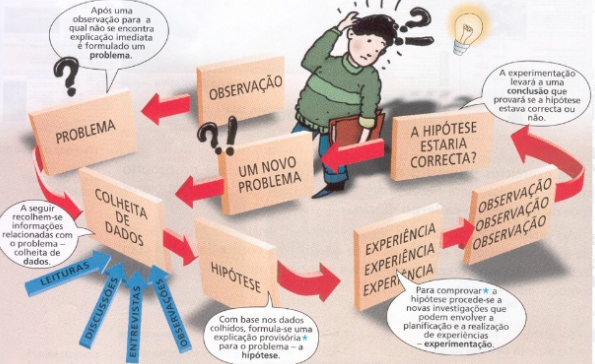
\includegraphics[scale=0.70]{Imagens/metodo.png}
%    \caption{Fases de uma pesquisa}
%    \label{metodo_cient}
% \end{figure}

%Uma lista completa das normas
%observadas pelo \abnTeX\ é apresentada em \citeonline{abntex2classe}.



% Este documento deve ser utilizado como complemento dos manuais do \abnTeX\ 
% \cite{abntex2classe,abntex2cite,abntex2cite-alf}. Consulte \citeonline{abntex2modelo} para obter
% exemplos e informações adicionais de uso de \abnTeX\ e de \LaTeX.






% ----------------------------------------------------------
% Elementos Textuais
% ----------------------------------------------------------
\chapter{Referencial Teórico}

\index{elementos textuais} Pretende-se fazer um Mapeamento Sistemático (MS) utilizando o Mapemento baseado em Problemas ou \textit{Problem Based Leaning} (PBL) aplicado à Ciência da Computação para obter a visão necessária da área pesquisada a fim de alcançar os objetivos determinados pelo tema. O PBL é uma metodoligia que utiliza problemas da vida real para desenvolver o processo de aprendizagem  \cite{Oliveira2012}.
Em certo modo Paulo Freire qualifica o desenvolvimento do processo de aprendizagem baseado nos problemas vivenciados pelo aprendiz \cite{Freire1987}. 



%
\begin{citacao}
O texto deve ser constituído de uma parte introdutória, na qual devem ser
expostos o tema do projeto, o problema a ser abordado, a(s) hipótese(s),
quando couber(em), bem como o(s) objetivo(s) a ser(em) atingido(s) e a(s)
justificativa(s). É necessário que sejam indicados o referencial teórico que
o embasa, a metodologia a ser utilizada, assim como os recursos e o cronograma
necessários à sua consecução.\citeonline{abntex2classe}
\end{citacao}

Deve-se apresentar a fundamentação teórica que orientará o estudo. Recomenda-se situar a grande área, subárea e objeto de estudo. Se for necessário pode ser feito um resgate histórico para demonstrar a evolução da área. Faz-se necessário relatar o momento vivido pela área (Marco Teórico - Estado da Arte) geralmente intitulado de Trabalhos Relacionados.

O Referencial Teórico é considerado como um elemento de controle de toda a pesquisa, desde a problematização inicial. O pesquisador irá interpretar seu objeto de estudo de acordo com a concepção teórica de uma ou toda a obra de um autor ou de um objeto ou produto ou de um conjunto de autores (esta condução varia de acordo com cada área de conhecimento). Todas as etapas do projeto são definidas conforme esta escolha. Apresenta-se de modo aprofundado, respondendo quais os princípios, categorias, conceitos ou teorias fundamentam a pesquisa. Deve estar de acordo com o tema formulado e o raciocínio desenvolvido nas fases anteriores. 


%===== Seção de Metodologia ==============

\chapter{Metodologia}

\index{elementos textuais} A fim de alcançar os objetivos na Seção Introdução \& Objetivos desta proposta, pretende-se desenvolver os trabalhos por meio das seguintes ações: 

\begin{enumerate}
\item
Pesquisa biblliográfica: Leitura de artigos e de livros que tratem do tema objeto da investigado. O passo inicial deverá acompanhar todo o desenvolvimento da tese. São exemplo de fontes importantes Pode-se fazer pesquisa bibliográfica nas seguintes fontes: IEEE Transactions on Systems, Man, and Cybernetics, Part C (Applications and Reviews), Elsevier Procedia -- Sicial and Behavioral Sciences,  
Pesquisa experimental: Desenvolvimento de um protótipo que permita o educador identficar em que nível estão seus educandos e agir pontualmente.
Estudo de caso: Aplicação da pesquisa em um ambiente escolar selecionado para comprovação dos resultados.
\item
	Universo, População e Amostragem:
O universo de pesquisa envolve os alunos do ensino medio da rede pública de ensino do Estado de Pernambuco bem como alunos do EJA. A rede pública de ensino em Pernambuco tem aproximadamente de 620 mil alunos, esta rede aumenta cerca de 15 mil novos alunos por ano  \cite{alunosEstado.2016}. Pretende-se fazer uma amostragem com 10\% desses alunos, ou cerca de 62 mil alunos. 
\item
	Coleta de Dados:
O dados coleta dos dados será realizada com autorização da Secretaria de Educação do Estado de Pernambuco.
\item
	Desenvolvimento e caracterização teórica:
A luz da teoria das ferramentas matemáticas e estatísticas que se pretende desenvolver com esta proposta deverá se fundamentar em tópicos de Mineração de Dados Educacionais, Mineração em Dados Textuais (Text Mining), ``Machine Learning'' e ``Deep Learning, ``E-learning'' e ``Leaning Analitycs''. O conhecimento sobre esses tópicos, a serem adquiridos na revisão bibliográfica e nas disciplinas cursadas devem possibilitar uma descrição formal e clara dos resultados obtidos ao longo dos estudos.
\item
	Ferramentas computacionais e simulações:
O estudo das ferramentas matemáticas desenvolvidas deve ser apoiado pelo uso de programas computacionais que facilitem implementações e permitam a realização de simulações das técnicas que vierem a ser propostas. Dentre esses programas, podem ser mencionados o R, o MYSql ou PostGreSQL, o Weka, além das linguagens de programação R, SQL, C/C++ e Python.
\item
	Acompanhamento do projeto:
O desenvolvimento do projeto deverá ser apoiado pelo orientador, por meio de reuniões presenciais semanais, pela participação do orientando como apresentador e ouvinte nos seminários quinzenais do Grupo de Pesquisa em Processamento de Sinais da UFPE. A ideia é que, ao final do doutorado, resultem do trabalho desenvolvido 04 artigos publicados em evento científico e 01 artigo publicado em periódico internacional.

\end{enumerate}
%===== Seção de Metodologia ==============

%\chapter{Cronograma}

%\index{elementos textuais}
%O cronograma tem por objetivo prever as ações distribuídas de acordo com o tempo previsto de pesquisa. O cronograma deve estar alinhado com os objetivos específicos e com a metodologia. Nos objetivos específicos tem-se “o que vou fazer”, na metodologia, “como vou fazer” e no cronograma, “quando vou fazer”.

%A  \autoref{tabela_cronog} apresenta o cronograma de execução da pesquisa. 

%\begin{table}[!htb]
%\centering
%\caption{Cronograma de Atividades}
%\label{tabela_cronog}
%\begin{tabular}{@{}llll@{}}
%\toprule
%\textit{Atividades}                  & \textit{Mês}       & \textit{Ano}   \\ \midrule
%Revisão Sistemática                  & Janeiro            & 2018           \\
%Análise de Trabalhos Relacionados    & Março              & 2018           \\
%Construção da Arquitetura            & Janeiro            & 2019           \\
%Implementação do Sistema             & Julho              & 2019           \\
%Avalição e Testes                    & Janeiro            & 2020           \\
%                                     &                    &                \\ \bottomrule
%\end{tabular}
%\end{table}




% ----------------------------------------------------------
% Capitulo com exemplos de comandos inseridos de arquivo externo 
% ----------------------------------------------------------

\include{abntex2-modelo-include-comandos}

% ---
% Finaliza a parte no bookmark do PDF
% para que se inicie o bookmark na raiz
% e adiciona espaço de parte no Sumário
% ---
\phantompart



% ----------------------------------------------------------
% ELEMENTOS PÓS-TEXTUAIS
% ----------------------------------------------------------
\postextual

% ----------------------------------------------------------
% Referências bibliográficas
% ----------------------------------------------------------
%\bibliographystyle{Bibliografia/Referencias.bib}
%\bibliography{abntex2-modelo-references}

\bibliography{Bibliografia/Referencias} % um arquivo (Bibliografia/Referencias.bib) está com as referências bibliográficas


% ----------------------------------------------------------
% Glossário
% ----------------------------------------------------------
%
% Consulte o manual da classe abntex2 para orientações sobre o glossário.
%
%\glossary

% ----------------------------------------------------------
% Apêndices
% ----------------------------------------------------------

% ---
% Inicia os apêndices
% ---
\begin{apendicesenv}

% Imprime uma página indicando o início dos apêndices
\partapendices

% ----------------------------------------------------------
\chapter{Exemplo de um apêndice A}
% ----------------------------------------------------------



% ----------------------------------------------------------
\chapter{Exemplo de um apêndice B}
% ----------------------------------------------------------


\end{apendicesenv}
% ---


% ----------------------------------------------------------
% Anexos
% ----------------------------------------------------------

% ---
% Inicia os anexos
% ---
\begin{anexosenv}

% Imprime uma página indicando o início dos anexos
\partanexos

% ---
\chapter{Exemplo de um primeiro anexo}
% ---


% ---
\chapter{Exemplo de um segundo anexo}
% ---



% ---
\chapter{Exemplo de um terceiro anexo}
% ---



\end{anexosenv}

%---------------------------------------------------------------------
% INDICE REMISSIVO
%---------------------------------------------------------------------

\phantompart

\printindex


\end{document}
